% !Mode:: "TeX:UTF-8"
% 文字编码:UTF-8
\chapter{延迟优化的实时视频码率自适应算法}
\label{chap:rate}

\section{引言}
随着移动智能设备和移动网络的普及,基于无线网络的实时视频通信的应用也越来越广泛。然而,在无线网络上进行实时视频传输还面临着带宽、延迟波动,物理链路丢包等挑战。为了避免网络拥塞引起的路由器主动丢包、延迟波动和带宽浪费,传统网络应用都需要采用TCP协议等对数据流进行拥塞控制。而在实时视频传输中,我们也必须要对视频流进行码率自适应。

视频传输码率自适应算法一直是一个活跃在学术界和工业界的热门问题,并且在TCP等传统拥塞控制算法的基础上发展出了不同的实现思路和方法。在第 \ref{chap:related}章,我们介绍了在网络传输尤其是实时视频传输过程中使用的主要码率自适应算法。本文从输入信号以及码率控制方式两个角度对主流实时视频码率自适应方法进行了分类。

首先,视频码率自适应算法作为一种网络拥塞控制算法,针对网络的负载状况反馈进行针对性的码率调整,必然要以网络真实参数作为输入信号,这些信号包括:
\begin{itemize}
    \item \textbf{丢包}:尽管无线网络由于信道质量差,发生丢包的概率较大,但丢包最主要的原因还是网络发生拥塞后在路由器上进行的主动丢包。因此,丢包也成为传统拥塞控制协议探测网络丢包的最主要手段。尽管如此,丢包信号应用在面向无线网络的数据传输中却并不合适。这是因为无线网络由于物理信道质量差,在没有网络拥塞的情况下丢包率也比较高,这会使拥塞控制算法低估网络带宽,造成带宽浪费。而且一旦网络拥塞引起了丢包,就说明网络已经发生了严重拥堵,这时延迟和抖动都非常严重,对实时视频通话效果的影响将需要很长时间恢复。
    \item \textbf{传输延迟}:数据从准备发送到成功接收之间的端到端延迟,通常用往返时延(Round Trip Time, RTT)衡量,主要包括:发送端数据处理、各中间路由器转发前的排队缓存、数据推送到传输介质以及数据在传输介质中传播四种不同延迟组成。其中唯一随网络状况有较大变化的就是数据包在中间路由器的排队缓存时间(我们称之为排队延迟),网络负载越大,缓存时间越长,排队延迟越大。因此,网络延迟也成为使用越来越多的拥塞控制信号。相对丢包而言,以网络延迟作为拥塞信号,可以根据延迟的增减情况判断网络状况的渐进变化,提前对视频码率进行调整以避免出现网络延迟,因而可以很好地保证视频数据传输的平稳高效。
    \item \textbf{抖动}:如果网络带宽、负载波动较大,就会使延迟出现较大波动,这一抖动尤其对延迟敏感的实时传输影响较大。因此延迟的相对抖动也成为视频码率自适应中需要参考的一种重要网络信号。
\end{itemize}
尽管在第 \ref{chap:related}章中提到的ECN标记也可以作为网络拥塞信号,但这类依赖于网络硬件参与的反馈信号需要对现有设备进行大规模改造,在通用算法中一般不予考虑。因此以上三条基本涵盖了主流拥塞控制算法所使用的反馈信号,当然在实际算法中可以综合利用其中的多种信号进行码率控制。

另外,从码率控制方式的角度进行总结,我们将主流拥塞控制算法分为以下三类:
\begin{itemize}
    \item 基于拥塞信号探测的控制。这类拥塞控制算法通过不断增加码率,直到网络达到某一可检测的阈值(例如丢包率达到某一阈值$P_{th}$\cite{wu2000end})来对网络带宽进行探测。常用的探测过程包括AIMD和MIMD 两种。这一控制方法通过控制网络保持在拥塞阈值之下来避免拥塞,但这一方法也导致网络延迟一直保持在较高水平。另外,当网络达到阈值时,为了避免即将发生的拥塞,必须大幅度降低发送速率(乘性减),因此发送码率波动较大,带宽利用率也相应较低。
    \item 基于网络模型的控制。与上述方法隐式估计网络带宽不同,基于模型的拥塞控制对网络建立公式描述,并计算相应的发送速率,以此显式地估计网络带宽。一种典型的应用是TFRC协议。一些基于控制论的方案也需要先建立网络控制模型,描述发送速率与网络参数之间的关系,从而建立闭环控制框图。
    \item 基于状态机的控制。随着视频通话应用不断涌现,在实际工程中一种基于状态机的算法应用越来越广泛。这一控制方法通过状态机对网络的不同状态进行描述,并通过一定条件触发状态间的转移。对于不同的网络状态,则采取不同的码率调整策略。通过对状态机的状态、跳转、行为等进行较细致的定义,可以给出比较复杂的控制系统,拟合不同的网络情境并充分结合应用测试中的经验。但这也成为该控制方法的一个缺点:模型和参数设定过分依赖工程经验,没有系统的优化方法,缺少理论支持。
\end{itemize}

我们的电视盒子视频通话系统主要应用场景是网络状况波动较大、丢包率较高的无线网络,在此背景下,大部分现有算法都不能对带宽进行有效利用。如基于丢包的算法存在带宽低估、延迟过大的问题;大部分算法都不能提供延迟波动范围的保证等。针对现有码率自适应算法的不足,我们希望设计一种针对无线网络实时视频传输的码率自适应算法,综合考虑无线网络高丢包的特点以及实时视频低延迟、稳定带宽的需求。这一算法的实现目标包括:
\begin{itemize}
    \item 在高丢包网络中准确估计真实带宽
    \item 稳定的低传输延迟
    \item 在带宽波动时反应灵敏、调整过程平滑
    \item 多流竞争公平性
\end{itemize}

为了实现上述目标,我们以控制论为基础,结合对网络排队延迟的建模,设计了一种延迟可控的视频码率自适应算法。首先,通过对带宽限制下的多流竞争系统建模和推导,我们引入了一个流式排队模型来对网络数据流的效率、稳定性、公平性进行分析。在这一流式排队模型中,通过控制排队延迟在一定范围内波动就可以完成网络拥塞控制。一种直观的理解是:当排队延迟超出预定值或增长过快时,通过及时降低视频码率来避免网络拥塞;当排队延迟低于预定值或下降过快时,通过提高视频码率来充分利用过剩的网络带宽。
我们将这一控制策略建模成非线性闭环控制模型,并对其进行线性化以利于进一步分析优化。最后,为了进一步提高系统性能,我们引入PID控制器,通过分析系统的稳定性和响应时间,对系统参数进行优化,从而为视频选择更加合适的码率。

%\section{带宽限制下的多流竞争分析}
%\label{section:shadow_price}
%
%在网络传输过程中,我们希望在有限的网络带宽限制下,为所有共享这一网络的用户提供更高的整体效用,这一问题可以用如下带约束的优化问题描述:
%\begin{equation}
%\label{eq:system_problem}
%\begin{aligned}
%& \max_{x_i}
%& & \sum_{i=0}^N{U(x_i)} \\
%& \text{s.t.}
%& & \sum_{i=0}^N{x_i} \leq C \\
%&&& x_i \geq 0, \; i = 1, \ldots, N.
%\end{aligned}
%\end{equation}
%$x_r$表示第$r$条数据流的发送速率,$U(x_r)$表示第$r$条流在发送速率$x_r$条件下获得的效用。所有数据流的发送速率$x_r$之和必须小于网络带宽$C$ 且不能为负数。
%在最优化问题中,拉格朗日乘数法是一种寻找多元函数在变量受到一个或多个条件的约束时的极值的方法。此问题中我们引入拉格朗日乘子$\lambda$并得到如下拉格朗日函数:
%\begin{equation}
%\label{eq:lagrangian}
%  \max L(x_i, \lambda) = \sum_{i=0}^N{U(x_i)} + \lambda (C-\sum_{i=0}^N{x_i})
%\end{equation}
%其中拉格朗日乘子$\lambda$也被称为影子价格。求解这一无约束形式的一阶条件包含如下约束:
%\begin{equation}
%\label{eq:FOC}
%  \frac{\partial L(x_i, \lambda)}{\partial x_i} = U'(x_r) - \lambda = 0
%\end{equation}
%
%在式 \ref{eq:FOC}中,由于我们还未给出$U(x)$的定义,因而暂时无法求解式 \ref{eq:system_problem}中的优化问题。根据常识可知,$U(x)$满足边际效用递减原理(即码率越大,增加单位码率对效用的提升越小),记为$U'(x) < 0$。 因此,尽管模型参数还未确定,我们可以使用渐进法逐步逼近$x$ 的准确值。渐进法形式如下:
%\begin{equation}
%\label{eq:approach}
%  x_i' = k ( U'(x_i) - \lambda)
%\end{equation}


\section{流式排队模型}
在以分组交换为基础的互联网数据传输中,用户数据被分割封装为包含了地址和管理信息的分组,分组通过最佳路径路由到目标,中间经过了路由器或交换机的层层转发。
以太网路由器的工作原理是存储转发,即先将输入端口到来的数据包缓存起来,按顺序对它们进行处理,因此也引入了较大的数据包处理延迟。
如果短时间内进入网络的数据包数量超出了网络的处理能力,就会在中间路由器堆积,形成网络拥塞。并进一步引起排队延迟增大,甚至路由器缓冲区溢出后发生大量丢包。

\begin{figure}[htbp]
  \centering
  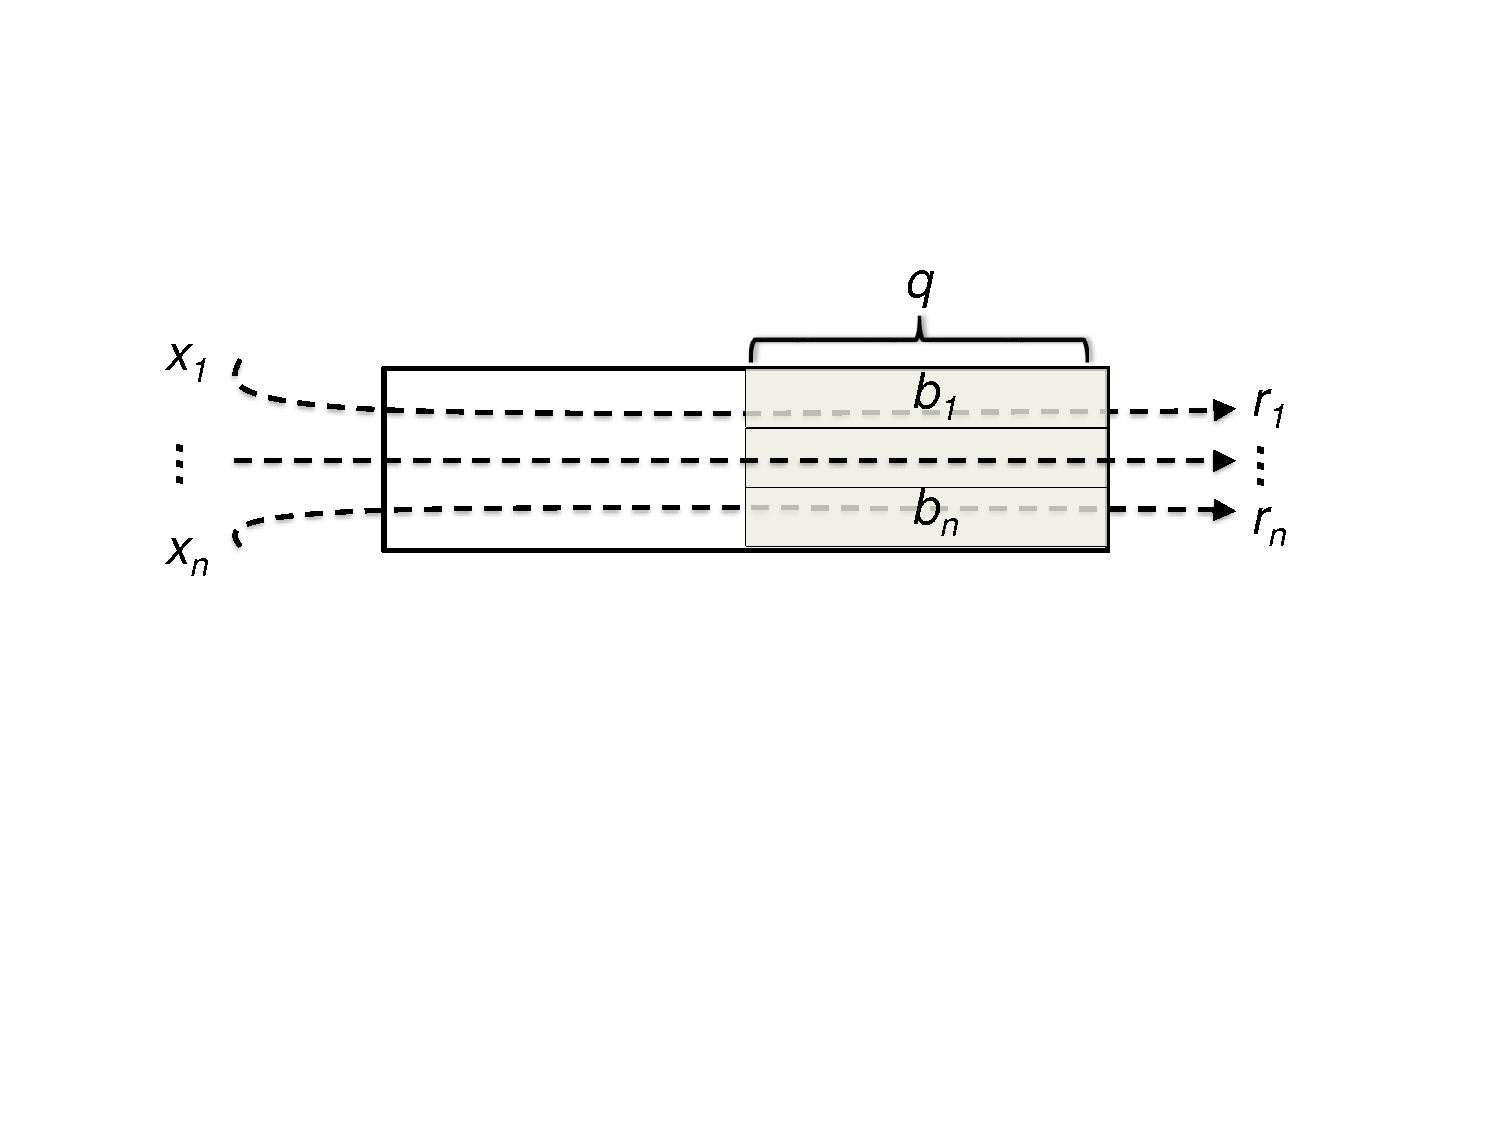
\includegraphics[width=0.5\textwidth]{buffer.pdf}
  \caption{流式排队模型}
  \label{fig:buffer}
\end{figure}

为了描述这一数据传输过程,我们通过图\ref{fig:buffer}所示的流式排队模型来对网络链路进行建模。我们将一条数据链路上的所有中间路由器简化为一个进行``存储-转发''的缓冲区,$N$ 个数据流在同一链路上进行数据传输,所有数据包都需要经过这一缓冲区才能达到目的地,因此形成对带宽资源的竞争。
假设第$i$ 条流占据的缓冲区数据量为$b_i$,其数据发送速率为$x_i$,从排队论的角度,整个缓冲区队列的入队速率为$\sum_{i=1}^N{x_i}$,其排空速率则始终等于网络带宽$C$。对于这一缓冲区的角度,有:
\begin{equation}
\label{eq:buffer}
  b'(t) = \sum_{i=1}^N{x_i(t)} - C
\end{equation}
其中 $b'(t)=db/dt$ 代表缓冲区大小随时间 $t$ 的变化速率。

图中 $q$ 表示前文提到的排队延迟,即数据包通过该缓冲区需要的时间。其含义为一个数据包进入缓冲区后,需要等待所有之前的数据包全部处理完毕才能通过缓冲区,这一过程即为``排队''。根据排队论,有:
\begin{equation}
\label{eq:delay}
    q(t) = \frac{b(t)}{C}
\end{equation}

考虑到单个网络流没有链路上的其他数据流的信息,为了达到系统的稳定公平,我们结合已有研究引入了基于影子价格 \cite{kelly1997charging}的码率控制模型。
首先根据视频数据的率失真曲线\cite{berger1971rate}赋予每条数据流权重 $\omega$,该权重值使每条视频数据流基于率失真公平性竞争带宽。如高清视频相对于普通视频具有更高的编码码率,因此可以设定较大的$\omega$以获得足够的带宽。
数据流对于获取的带宽需要付出价格为 $p(t)$ 的拥塞代价。利用失真权重和影子价格的码率控制模型可以描述为
\begin{equation}
\label{eq:rate}
    x_i'(t) = \omega_i - x_i(t)p_i(t)
\end{equation}
其中 $x_i'(t)=dx_i/dt$ 代表码率随时间的变化速率。

所有视频流根据式\ref{eq:rate}调整视频码率。当网络接近拥塞时,码率较高的视频流由于付出更大的拥塞代价,码率下降更快。经过一段时间的动态调整,所有视频流都稳定在失真公平的码率附近。与直接参考传输延迟的值进行码率控制的 FAST TCP\cite{wei2006fast} 等协议不同的是,我们以拥塞代价$p(t)$作为中间值,解耦了码率控制和延迟之间的直接关系,从而使调节过程更加灵活,避免了调节过程中的延迟积累、波动等问题。


\section{闭环码率控制模型及其线性化}
在实际应用场景中,不同用户进行视频通话的质量各不相同,而他们之间带宽竞争的公平性在不同衡量标准(如使用带宽分配情况、视频清晰度、用户满意程度)下具有不同的结果,这本身就是一个值得研究的问题。在本文中,为了简化分析过程,我们假设所有用户是同质的,即他们具有同样的视频权重 $\omega$ ,因而系统稳定状态下,每个人获得的发送速率$x$也应该相等。这样式\ref{eq:buffer}-\ref{eq:rate}可以简化为
\begin{equation}
\label{eq:rate_model}
\left\{\begin{array}{l}
    x' = \omega - xp \\
    b' = Nx - C\\
    q = \frac{b}{C} + t_p
\end{array} \right.
\end{equation}

从控制论的角度看,上述系统是一个分析难度很大的非线性系统。为了简化分析,我们在其稳定点取差分,从而将其等效转化为线性系统。记其稳定点的影子价格为$p_0$,对应发送速率为$x_0$,且稳定点满足$x'=0$,则:
\begin{equation}
x'=0 \Longrightarrow \left\{\begin{array}{l}
    \omega = x_0 p_0\\
    x_0 = \frac{C}{N}
\end{array} \right.
\end{equation}

\begin{figure}[htbp]
  \centering
  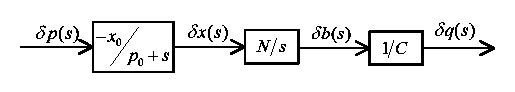
\includegraphics[width=0.7\textwidth]{block2.eps}
  \caption{复数域控制系统框图}
  \label{fig:block2}
\end{figure}

对各参数进行差分操作$\delta p(t)=p_0 - p(t)$, $\delta x(t) = x_0 - x(t)$ 和 $\delta q(t) =q_0 - q(t)$,得到线性化之后的码率控制系统如下:
\begin{equation}
\label{eq:linear}
\left\{\begin{array}{l}
    \delta b'(t) = \sum_{i=1}^{N}{\delta x(t)}  \\
    \delta q(t)  = \frac{\delta b(t)}{C} \\
    \delta x'(t) = -p_0\delta x(t) - x_0 \delta p(t)
\end{array} \right.
\end{equation}
根据控制论对式 \ref{eq:linear} 进行拉普拉斯变换,得到该控制系统在复数域的控制框图如图\ref{fig:block2}所示。

\begin{figure}[htbp]
  \centering
  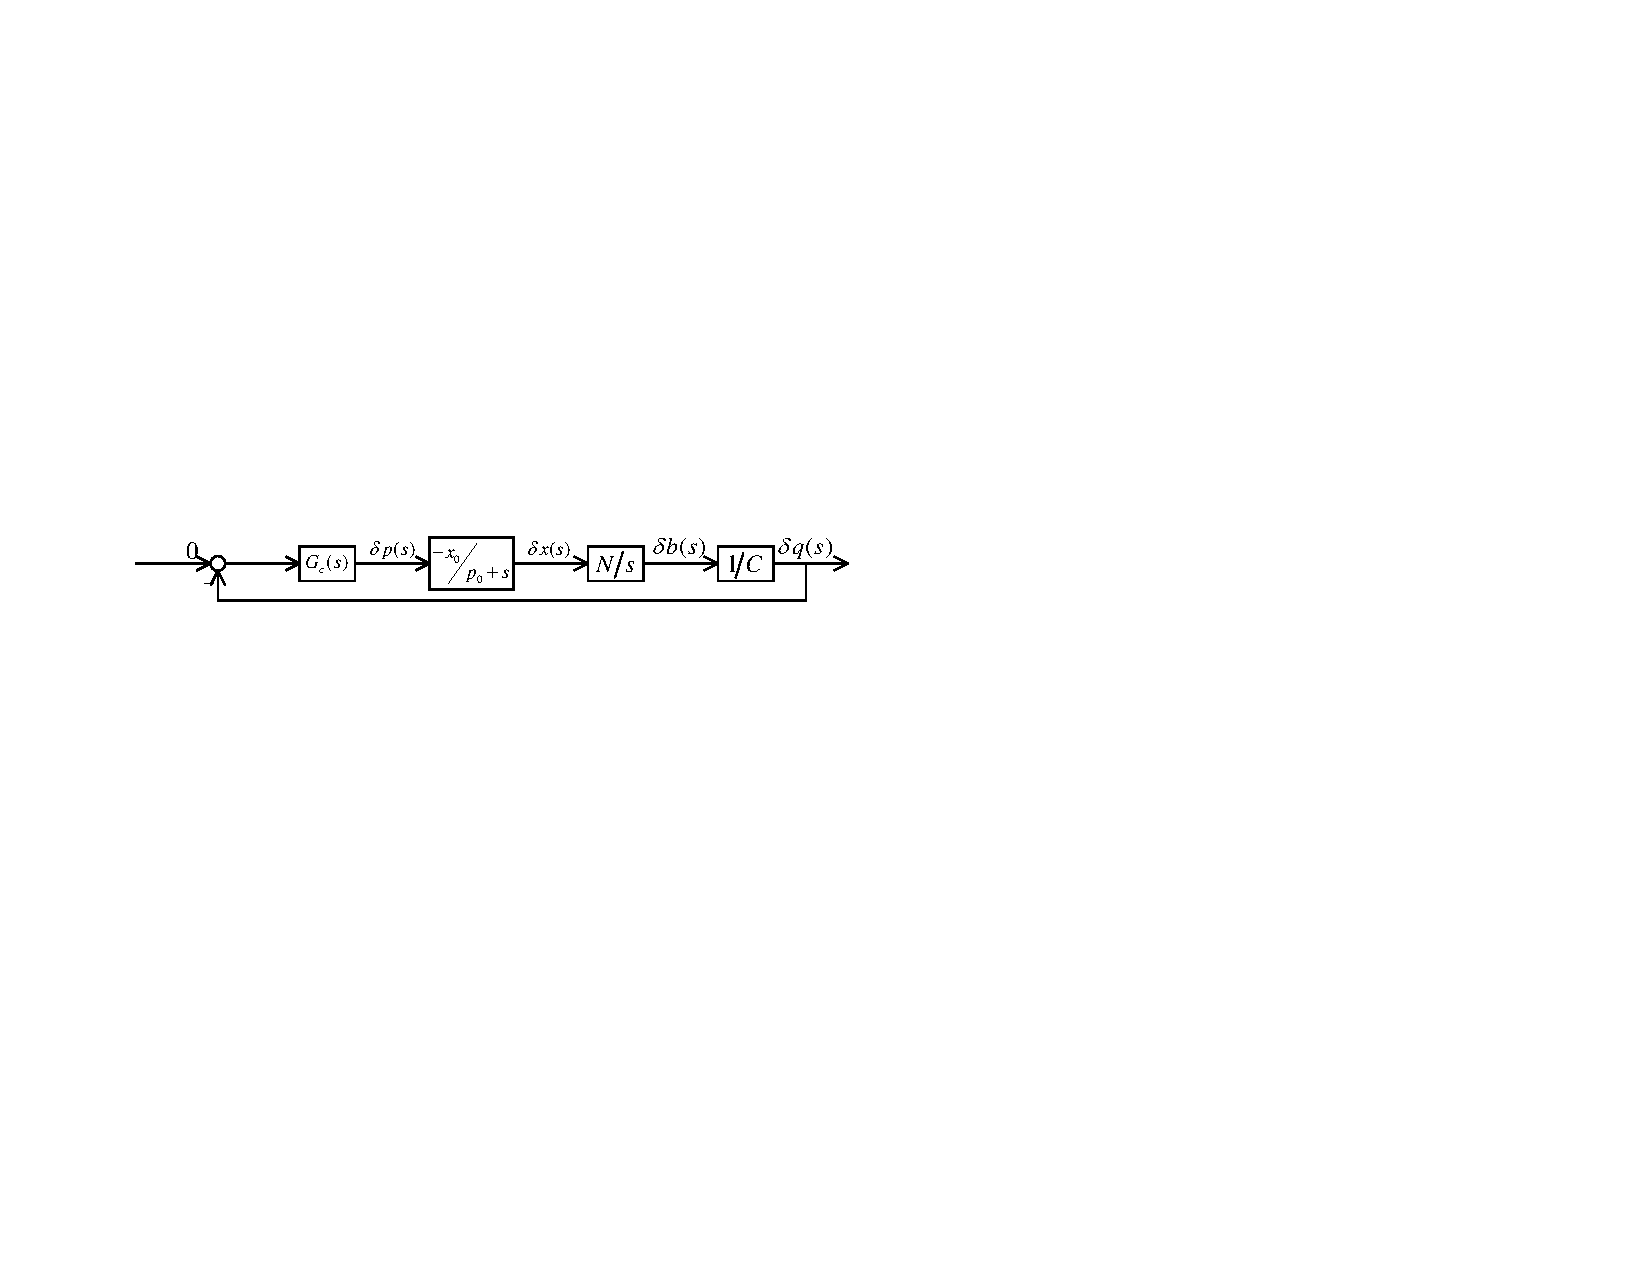
\includegraphics[width=0.8\textwidth]{block3.pdf}
  \caption{闭环控制系统框图}
  \label{fig:block3}
\end{figure}

显然上述控制模型还没有形成闭环控制逻辑,其中缺失的关键环节就是系统输出的排队延迟与系统输入的拥塞代价之间的关系。
前文已经提到,拥塞代价是排队延迟与视频码率这一对控制变量之间插入的中间变量,在该控制模型中,我们的主要目标是以排队延迟作为系统反馈,来控制数据流的影子价格$p$,进而根据式 \ref{eq:rate}决定视频码率。根据图\ref{fig:block2}及控制论知识,我们在控制框图中添加一个以$\delta q(s)$为输入,$\delta p(s)$为输出的控制器$G_c(s)$
\begin{equation}
\delta p(s) = G_c(s)\delta q(t)
\label{equ_x_dif}
\end{equation}
完成这一控制过程,从而形成一个如图 \ref{fig:block3}所示的闭环反馈控制系统。

\section{PID控制器设计}
PID(比例-积分-微分)控制器是一种反馈回路部件,经常应用在工业控制系统中。这个控制器把收集到的数据和一个参考值进行比较,然后把这个差别用于计算新的输入值,这个新的输入值的目的是可以让系统的数据达到或者保持在参考值。PID控制器可以根据历史数据和差别的出现率来调整输入值,使系统更加准确而稳定。

PID控制器的比例单元P、积分单元I和微分单元D分别对应目前误差、过去累计误差及未来误差。在本文中,综合考虑控制效果和系统求解复杂度,我们选择比例控制器作为$G_c(s)$的实现,即
\begin{equation}\label{eq:gcs}
    G_c(s) = K_P
\end{equation}

不同的$K_P$取值决定了整个控制系统能否稳定,以及系统的响应时间等重要性能。为了对此进行分析,我们结合图\ref{fig:block3}和式\ref{eq:gcs}推导出该闭环控制系统的转移方程如下:
\begin{equation}\label{eq:transfer}
    H(s) = \frac{K_P}{s^2 + s p_0 + K_P} = \frac{\omega^2}{s^2 + 2 \zeta \omega s + \omega^2}
\end{equation}
其中$\zeta$代表系统的阻尼比,描述系统在受到扰动后振荡及衰减的情形。$\omega$代表系统的固有频率,即系统受到扰动后在无阻尼条件下的振荡频率。由上式可知$2 \zeta \omega = p_0$ 且$\omega^2 = K_P$,从而得到$\zeta = \frac{p_0}{2\sqrt{K_P}}$。为了得到良好的系统响应,我们选择已被证明具有较好系统表现的阻尼比$\zeta = \frac{\sqrt{2}}{2}$\cite{franklin2006feedback},则有
\begin{equation}\label{eq:k}
    K_P = \frac{p_0^2}{2}
\end{equation}
在以上取值条件下,系统的$5\%$稳定时间$T_s = \frac{6}{p_0}$。即当系统发生随机扰动后,在不超过$\frac{p_0^2}{2}$的时间内,系统可以调整到与目标码率差值不超过$5\%$的码率范围内,因此通过恰当的参数取值,可以保证系统的响应速度。


\section{实现细节说明}
为了方便地测试本文提出的码率自适应算法的效果,以及与现有算法的性能对比,我们基于前述开源软件Linphone的底层视频传输模块——Mediastreamer2,搭建了算法测试平台。基于视频码率自适应算法,我们实现了一个包含网络信息采集和发送、最优码率计算等功能的码率自适应模块。除此之外的大部分功能(如视频采集、码率可变编解码等)都沿用了已有实现。本节中,我们简要介绍一些系统实现中的重要细节。

    \subsection{排队延迟的计算}\label{chap:qd_calc}
    在数据传输过程中,传输延迟定义为数据包从发送端开始发送到接收端成功接收之间的时间间隔。其直观测量方式就是对数据包发送和接收时刻分别获取当前时间并作差,这一差值定义为单向延迟(One Way Delay, OWD)。然而,由于发送和接收两个客户端的时间设置很难保证完全同步,在单向延迟的计算中一个无法排除的误差就是时钟偏差。因此,在实际网络应用中,衡量网络延迟使用的一般是往返时延(Round-Trip Time, RTT)这一变量,表示从发送端发送数据开始,到发送端收到来自接收端的确认(接收端收到数据后便立即发送确认),总共经历的时延。

    在视频通话过程中,视频流是双向同时进行的,但由于网络环境的多样性,不同方向上的网络状况可能存在很大区别。如果采用RTT作为延迟信号,我们只能获得上下行两个方向上的延迟之和,因而无法针对单向链路进行针对性的码率调整。在本研究中,利用即将给出的排队延迟的特性,我们可以消除单向延迟存在时钟偏差的问题,因而可以采用单向延迟进行更加精确的码率调整。

    由单向延迟的定义我们知道
    \begin{equation}\label{eq:owd}
        OWD = D_q + D_t
    \end{equation}
    其中$D_q$为排队延迟,$D_t$为除排队延迟以外的其他延迟,这部分延迟主要与网络物理环境有关,因此连接建立后变动很小。因此,我们可以通过如下方式计算排队延迟
    \begin{equation}\label{eq:qd}
        D_q = OWD - OWD_{min}
    \end{equation}
    其中$OWD_{min}$是传输过程中单向延迟的最小值,在每次计算单向延迟时更新。考虑到当网络负载达到最小时,数据包在所有路由器上都直接被处理,则其延迟中将不包含排队延迟,我们认为这一最小值可以很好地估计网络的固定时延。同时在对单向延迟作差的过程中,我们已经消除了时钟偏差这一误差。

    \subsection{影子价格的更新}
    由式 \ref{eq:gcs}定义的比例控制器,有
    \begin{equation}\label{eq:kpt}
        \delta p = K_P \delta q
    \end{equation}
    在系统实现角度,由于不同的视频流特性、网络状况等,不同系统具有不同的系统取值,我们不可能提前知道任一系统达到稳态时对应的影子价格$p_0$。然而注意到上式中排队延迟和影子价格都是差分形式,将其展开后有:
    \begin{equation}
        p(t) = p(t-1) + K_p(q(t) - q(t-1))
    \end{equation}
    通过这一变形,我们可以在系统运行过程中逐步逼近正确的影子价格。同时根据式\ref{eq:k}动态更新相应的$K_P$值。

    \subsection{视频码率控制}
    式 \ref{eq:rate}给出了时间连续的系统中码率的变化率公式,然而在实际系统中,调整间隔不可能无限小。我们去单词码率调整的时间间隔为$\Delta{T}$,则在此离散的码率调整方式下码率计算公式为
    \begin{equation}
        x(t) = x(t-1) + x'(t) \Delta{T}
    \end{equation}

    我们在每个时间片起始时更新视频码率。系统启动时,视频码率被设定为编码器允许的最小值,如64Kbps。


\section{实验验证}
本小节中,我们基于实验平台对我们的码率自适应算法进行了测试,并与几种主流拥塞控制算法进行了对比。

    \subsection{实验设置}

    \begin{figure}[htbp]
      \centering
      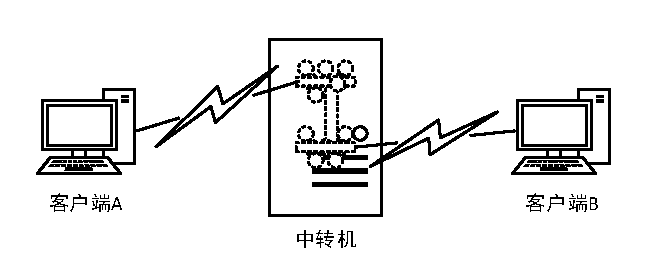
\includegraphics[width=0.7\textwidth]{rate_exp_arch.pdf}
      \caption{测试平台设置}
      \label{fig:rate_exp_arch}
    \end{figure}

    如图 \ref{fig:rate_exp_arch},我们用三台主机组成测试平台,其中一台作为中转机,另外两台主机分别作为发送端和接收端与中转机连接。由于两台客户端分别连接了中转机的不同网卡,因此它们的数据通信必须经过中转机转发,我们可以通过中转机上运行的带宽控制软件Network Emulator for Windows Toolkit (NEWT) 来对网络链路进行仿真模拟,包括带宽限制、丢包控制和背景延迟控制等,同时可以实时监测网络带宽的分配和利用情况。

    通过理论分析和实验测试,我们对部分参数的取值进行了优化。如码率调整的时间间隔$\Delta T$设置为300ms。为了平衡带宽利用率和延迟约束,将目标排队延迟设置为$q_0 = 100$ms。

    在对比测试中,我们选择了经典的基于模型的码率控制算法TFRC协议,和基于AIMD 控制的CTCP \cite{song2006compound} 协议。其中TFRC协议通过一个关于丢包率和RTT的函数来计算发送速率,而CTCP 协议作为基于探测的拥塞控制的代表,通过加性增长,乘性降低来隐式估计网络带宽。我们在上述Mediastreamer系统中对这三种码率自适应算法全部进行了实现。

    在本研究的实验验证中,我们主要关注码率自适应算法在三方面的表现,分别是数据传输质量、数据分配公平性和视频服务质量。
    其中数据传输质量通过平均视频码率和码率稳定性来衡量。平均视频码率取通话开始60s之后至通话结束码率自适应算法输出的目标码率平均值,码率稳定性通过这些目标码率的标准差衡量,公式如下:
    \begin{displaymath} \label{eq:throughput}
    Stability = \frac{1}{\bar{x}}\sqrt{ \frac{1}{n} \sum_{i=1}^{n}(x_i-\bar{x})^2 }
    \end{displaymath}
    %代表传输质量的平均码率和码率稳定性,同算法间码率分配公平性,以及代表服务质量的PSNR。 其中平均码率在接收端码率稳定60s之后开始记录。码率稳定性通过码率的标准差衡量如下
    码率分配公平性通过多流竞争条件下的不同视频流的码率动态关系进行评价。
    视频服务质量通过接收端观看视频与原始视频的质量差异大小衡量,其通用的衡量方法是PSNR。即通过比较发送端的输入CIF序列和接收端解码的CIF序列计算得到的PSNR值。

    \subsection{结果分析}

        \subsubsection{平均码率和码率稳定性}

        \begin{figure}[htbp]
          \begin{subfigure}[b]{0.5\textwidth}
            \centering
            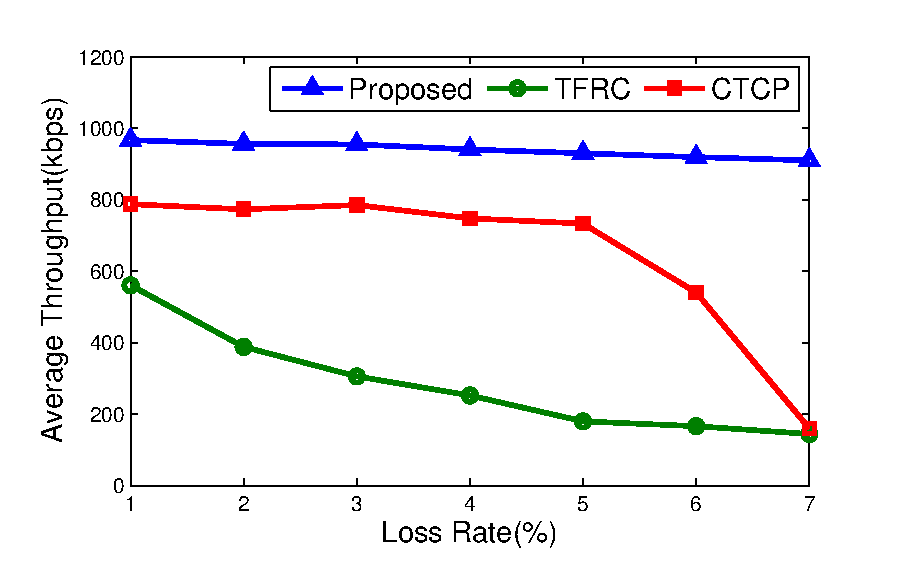
\includegraphics[scale=0.5]{lossrate_bw.eps}
            \caption{平均码率表现}
            \label{pic:lossrate_bw}
          \end{subfigure}
          \begin{subfigure}[b]{0.5\textwidth}
            \centering
            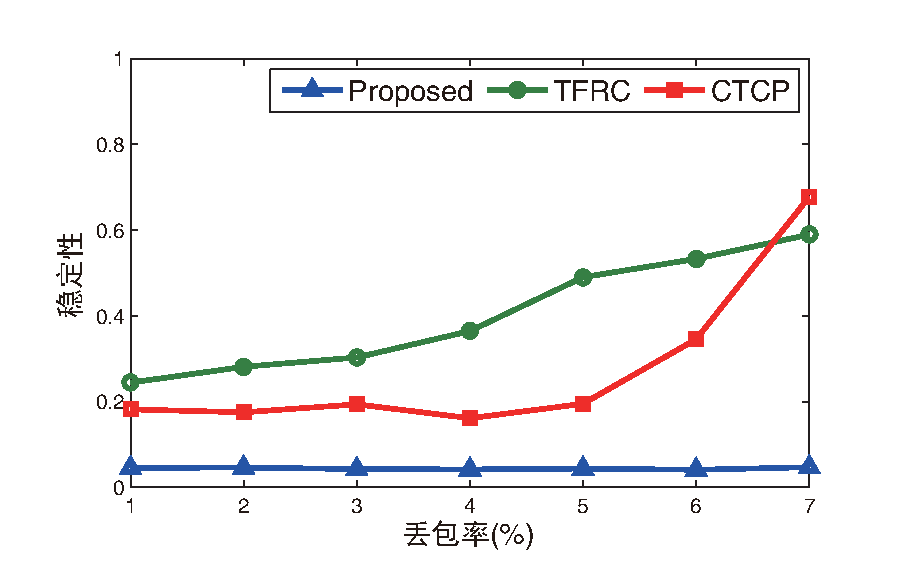
\includegraphics[scale=0.5]{lossrate_st.eps}
            \caption{码率稳定性表现}
            \label{pic:lossrate_st}
          \end{subfigure}
          \caption{不同丢包率下算法表现,带宽=1Mbps,背景延迟=50ms}
          \label{pic:lossrate}
        \end{figure}

        我们首先对平均码率和码率稳定性在不同算法间进行测试。图\ref{pic:lossrate}展示了不同丢包率的网络场景。可以看出我们的算法始终具有更好的表现。这主要由于我们的算法使用排队延迟而不是丢包作为网络拥塞信号,使其能够排除网络固有丢包对拥塞判断的影响。另外得益于控制论参数优化,尽管丢包率不断增大,我们的算法仍保持了较好的平均码率和码率稳定性水平。

        \begin{figure}[htbp]
          \begin{subfigure}[b]{0.5\textwidth}
            \centering
            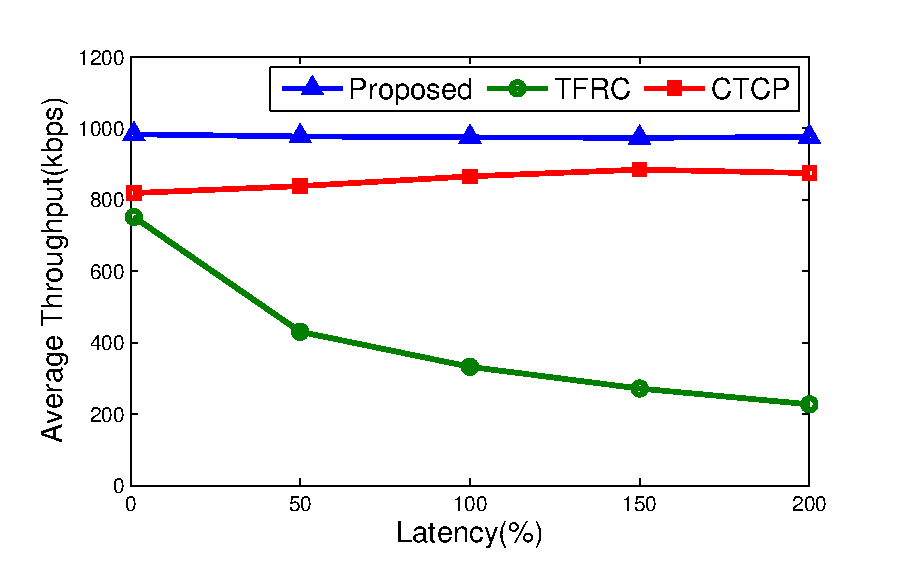
\includegraphics[scale=0.5]{latency_bw.eps}
            \caption{平均码率表现}
            \label{pic:latency_bw}
          \end{subfigure}
          \begin{subfigure}[b]{0.5\textwidth}
            \centering
            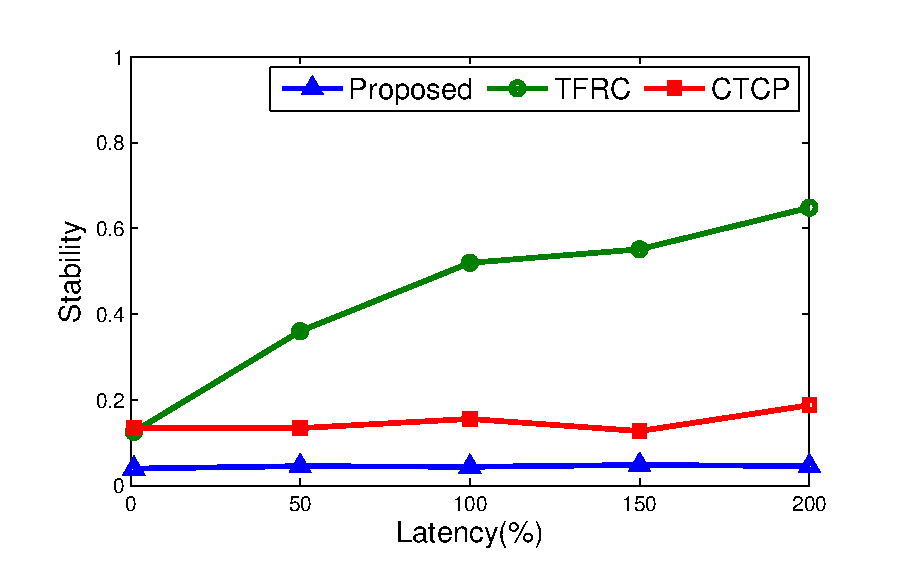
\includegraphics[scale=0.5]{latency_st.eps}
            \caption{码率稳定性表现}
            \label{pic:latency_st}
          \end{subfigure}
          \caption{不同背景延迟下算法表现,带宽=1Mbps,丢包率=1\%}
          \label{pic:latency}
        \end{figure}

        同时,我们比较了不同背景延迟条件下几种算法的表现,结果如图\ref{pic:latency}。从结果中可以看到,当延迟水平比较低时,所有算法都能得到较大的平均码率,随着延迟增大,基于延迟进行控制的TFRC算法平均码率急剧下降,而CTCP算法由于不考虑延迟变化,因此不受影响。我们的算法通过延迟优化,始终能保持较高的平均码率和较好的码率稳定性。

        \begin{figure}[htbp]
          \begin{subfigure}[b]{0.5\textwidth}
            \centering
            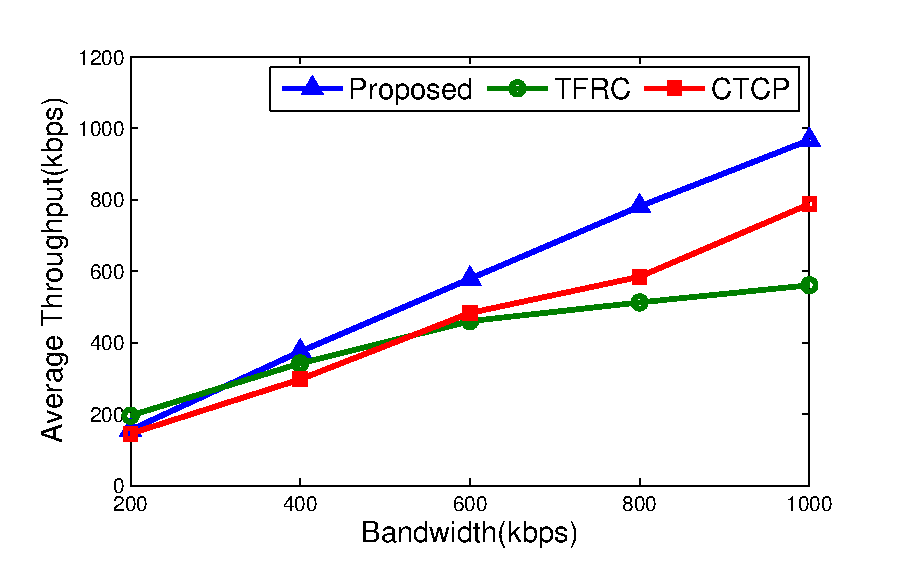
\includegraphics[scale=0.5]{bandwidth_bw.eps}
            \caption{平均码率表现}
            \label{pic:bandwidth_bw}
          \end{subfigure}
          \begin{subfigure}[b]{0.5\textwidth}
            \centering
            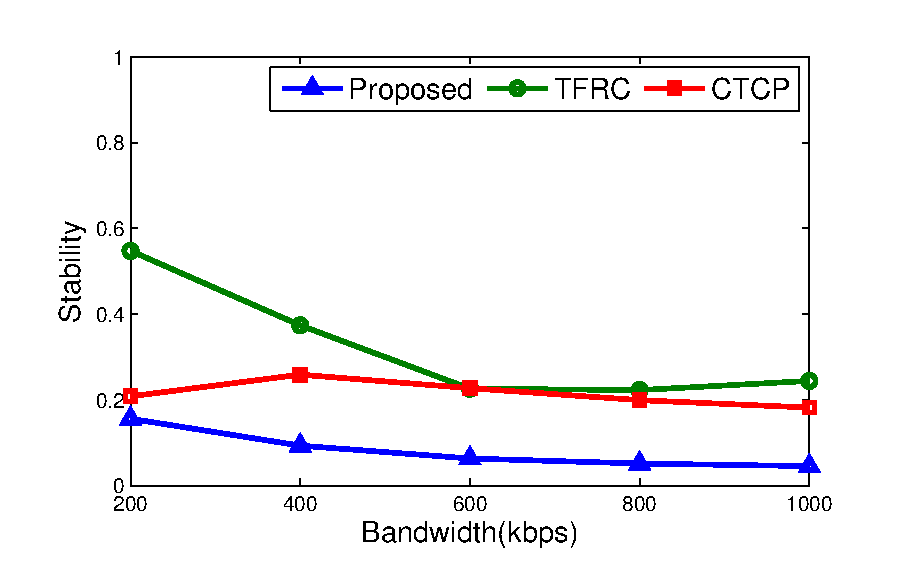
\includegraphics[scale=0.5]{bandwidth_st.eps}
            \caption{码率稳定性表现}
            \label{pic:bandwidth_st}
          \end{subfigure}
          \caption{不同带宽限制下算法表现,丢包率=1\%,背景延迟=50ms}
          \label{pic:bandwidth}
        \end{figure}

        最后,我们比较了不同网络带宽限制下几种算法的表现,如图 \ref{pic:bandwidth}。与前几项实验结果相同,我们的算法在不同环境中均表现出更好的效果。由于我们采用了排队延迟作为码率调整的主要信号,因而可以提前发现网络状况的波动,并通过改变码率来逼近实际带宽。另外得益于我们利用控制论进行的参数优化,保证了我们的码率自适应算法过程更加平滑、结果更加准确。

        \subsubsection{动态公平性}
        \begin{figure}[htbp]
          \centering
          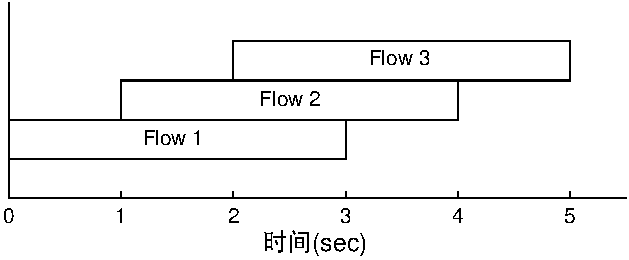
\includegraphics[width=0.6\textwidth]{flows.pdf}
          \caption{多流动态模型}
          \label{pic:flows}
        \end{figure}

        \begin{figure}[htbp]
          \centering
          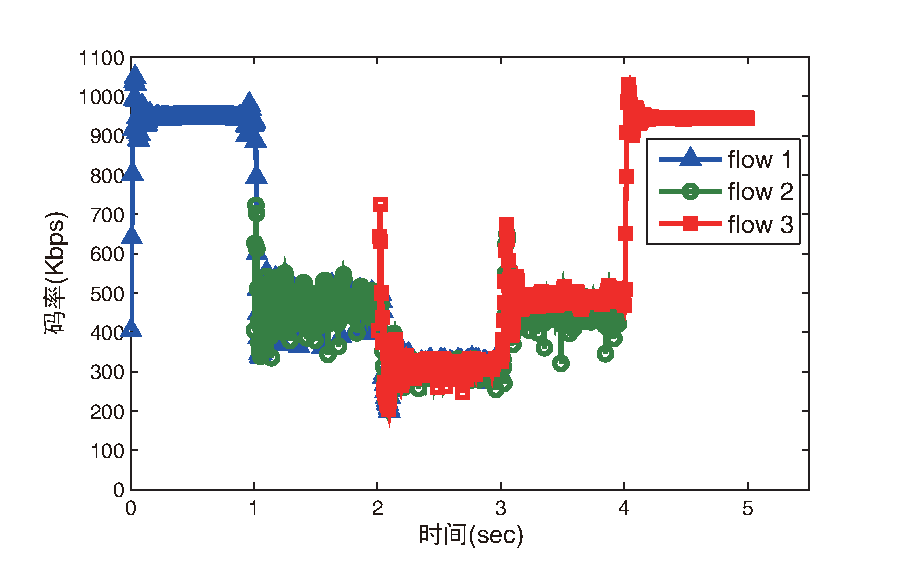
\includegraphics[width=0.7\textwidth]{flows_bw.eps}
          \caption{动态码率变化}
          \label{pic:flows_bw}
        \end{figure}

        除了静态网络中的测试以外,码率自适应算法在动态网络中能否迅速反应带宽变化也是评价的重要标准。本项测试中,我们选择三条数据流分别在不同时间启动和终止,如图\ref{pic:flows} 所示。在发送端,我们记录每条流的动态视频码率,结果如图\ref{pic:flows_bw}。 结果表明,我们的算法对网络波动反应迅速准确,并且每条流都能获取的均等大小的网络带宽。

        \subsubsection{视频质量}
        \begin{figure}[htbp]
          \centering
          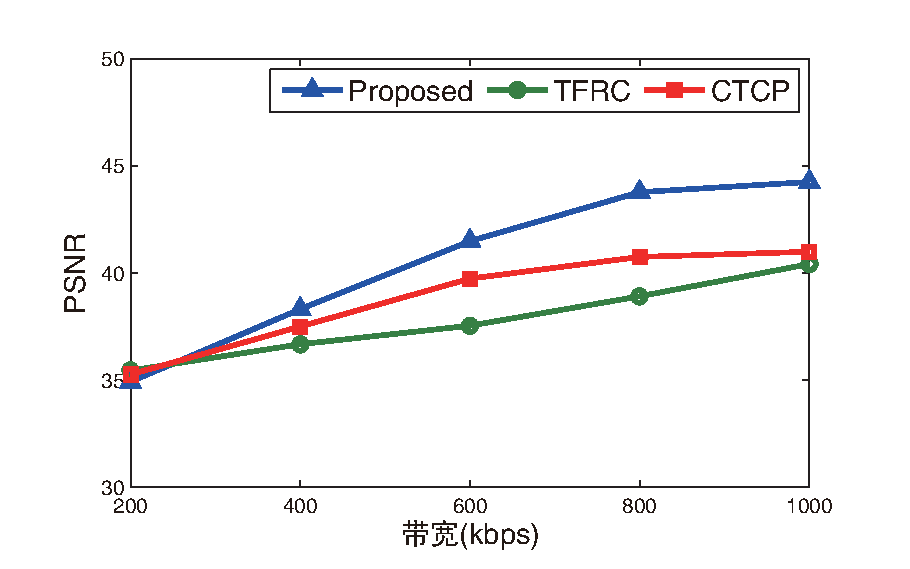
\includegraphics[width=0.7\textwidth]{psnr.eps}
          \caption{不同带宽限制下视频质量表现,丢包率=1\%,延迟=50ms}
          \label{pic:psnr}
        \end{figure}

        最后,我们比较了不同带宽限制下,三种码率自适应算法在接收端视频的PSNR质量表现,结果如图\ref{pic:psnr}所示。可见我们的算法在不同带宽下均能获得视频质量的显著提升。这主要得益于我们使用的比例控制器优化,及基于排队模型的延迟优化,使其能够获得更高的平均码率和码率稳定性。


\section{本章小结}
本章中,我们针对无线网络中的实时视频传输,提出了一个分布式、延迟可控的码率自适应算法,满足了视频传输中的低延迟、带宽稳定、高带宽利用率等需求。我们首先通过对网络建模分析,提出了简化网络链路的排队延迟模型,并引入了影子价格和失真权重参数来更好地实现拥塞控制和多流公平。通过建立闭环反馈控制模型,并引入比例控制器进行参数优化,使得控制过程更加高效、平滑。另外,我们在开源系统的基础上对几种码率自适应算法进行实现,并进行了大量效果测试。实验表明,相比于其他主流码率自适应算法,我们的算法在带宽利用率、稳定性,视频质量等方面都有更好的表现。
